% Nallino, Part I p. 102: the figure of a lunar eclipse, redrawn from the print: the horizon ABCD
% (centre F) with the lines AC and BD, the circle of the half sum of the diameters (through P), the
% circle of the shadow, the three discs of the Moon (centres M, on AC, K), the lines ML, MK, MF, HK,
% FK, FQ and FT; the four quarters MERIDIES, SEPTENTRIONES, ORIENS (reading downward) and OCCIDENS
% (reading upward). Circles and lines are least-squares fits to the printed ink; coordinates are
% PDF points of master page 191 less the origin (106.56, 348.56), y downward.
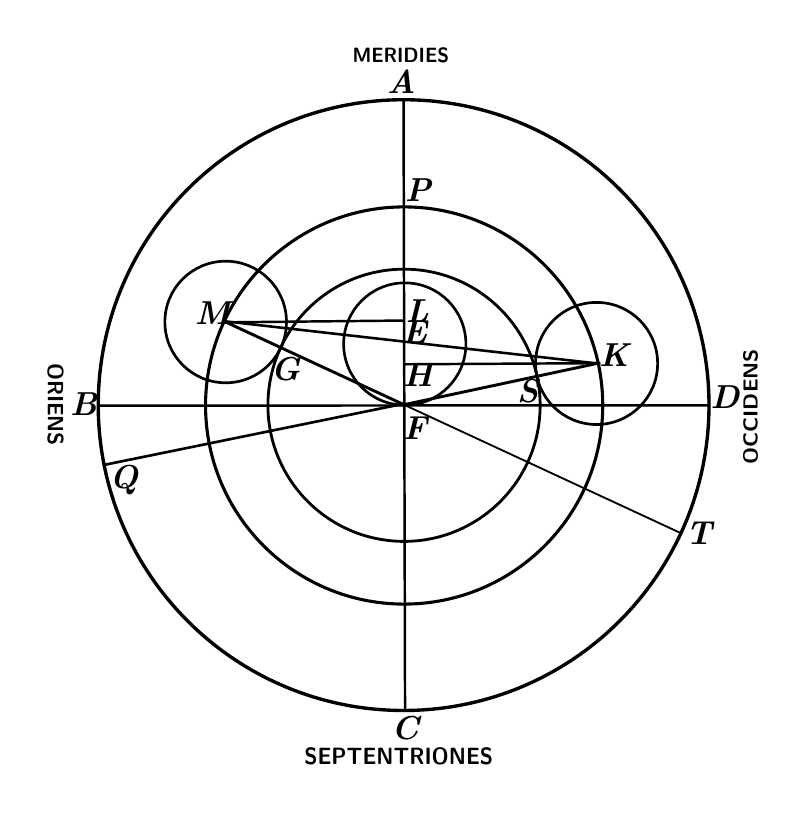
\begin{tikzpicture}[x=0.9942pt,y=-0.9942pt,line cap=butt,every node/.style={font=\fontsize{11.5}{11.5}\bfseries\itshape\selectfont,inner sep=0pt}]
\useasboundingbox (0,0) rectangle (270.00,276.00);
\draw[line width=1.22pt] (136.64,137.18) circle[radius=110.99];  % the horizon ABCD, centre F
\draw[line width=1.12pt] (136.83,137.32) circle[radius=72.18];  % the circle of the half sum of the two diameters, through P
\draw[line width=1.02pt] (136.79,137.24) circle[radius=49.47];  % the circle of the shadow
\draw[line width=0.97pt] (71.96,106.97) circle[radius=22.10];  % the Moon at the beginning of the immersion, centre M
\draw[line width=0.96pt] (137.06,114.97) circle[radius=22.22];  % the Moon at the middle of the eclipse
\draw[line width=0.97pt] (206.77,122.04) circle[radius=22.19];  % the Moon at the end of the emersion, centre K
\draw[line width=0.89pt] (136.61,26.20) -- (137.16,248.17);  % the line AC (south to north)
\draw[line width=0.89pt] (25.66,137.38) -- (247.63,137.25);  % the line BD (east to west)
\draw[line width=0.89pt] (70.92,107.11) -- (136.81,106.44);  % the line ML
\draw[line width=0.93pt] (71.19,106.66) -- (208.19,122.18);  % the line MK
\draw[line width=1.05pt] (71.25,106.66) -- (136.88,137.08);  % the line MF
\draw[line width=0.89pt] (136.85,122.34) -- (207.91,121.94);  % the line HK
\draw[line width=1.05pt] (136.88,137.01) -- (207.82,121.85);  % the line FK
\draw[line width=0.95pt] (136.88,136.65) -- (27.80,158.91);  % the line FQ
\draw[line width=0.67pt] (136.88,137.09) -- (237.40,183.71);  % the line FT
\node at (135.74,19.74) {A};
\node at (141.82,59.14) {P};
\node at (67.20,103.75) {M};
\node at (141.59,103.04) {L};
\node at (140.54,110.59) {E};
\node at (93.70,124.09) {G};
\node at (141.74,126.19) {H};
\node at (213.09,118.83) {K};
\node at (181.72,132.01) {S};
\node at (20.32,136.72) {B};
\node at (253.40,134.17) {D};
\node at (140.79,145.64) {F};
\node at (34.99,164.62) {Q};
\node at (243.96,183.75) {T};
\node at (137.19,254.66) {C};
\node at (135.62,9.97) {\normalfont\fontsize{8.5}{8.5}\sffamily\bfseries\selectfont \resizebox{34.90pt}{5.19pt}{MERIDIES}};
\node at (134.88,264.67) {\normalfont\fontsize{8.5}{8.5}\sffamily\bfseries\selectfont \resizebox{68.18pt}{5.91pt}{SEPTENTRIONES}};
\node[rotate=-90] at (10.13,136.93) {\normalfont\fontsize{8.5}{8.5}\sffamily\bfseries\selectfont \resizebox{29.89pt}{5.55pt}{ORIENS}};
\node[rotate=90] at (262.77,137.75) {\normalfont\fontsize{8.5}{8.5}\sffamily\bfseries\selectfont \resizebox{41.61pt}{5.10pt}{OCCIDENS}};
\end{tikzpicture}
